\documentclass[8pt]{extarticle}
\title{Econ 250 HW 7}
\author{Avinash Iyer}
\date{}

%font setup
%
%\usepackage[math]{anttor}

%paper setup
\usepackage{geometry}
\geometry{letterpaper, portrait, margin=1in}
\usepackage{fancyhdr}
\usepackage{enumitem}

%symbols
\usepackage{amsmath}
\usepackage{amssymb}
\usepackage{hyperref}
\usepackage{gensymb}

\usepackage[T1]{fontenc}
\usepackage[utf8]{inputenc}

%chemistry stuff
\usepackage[version=4]{mhchem}
\usepackage{chemfig}

%plotting
\usepackage{pgfplots}
\usepackage{tikz}

%\usepackage{natbib}

%graphics stuff
\usepackage{graphicx}
\graphicspath{ {./images/} }

%a useful command
\newcommand{\plain}[1]{\textrm{#1}}

%code stuff
%when using minted, make sure to add the -shell-escape flag
%you can use lstlisting if you don't want to use minted
%\usepackage{minted}
%\usemintedstyle{pastie}
%\newminted[javacode]{java}{frame=lines,framesep=2mm,linenos=true,fontsize=\footnotesize,tabsize=3,autogobble,}
%\newminted[cppcode]{cpp}{frame=lines,framesep=2mm,linenos=true,fontsize=\footnotesize,tabsize=3,autogobble,}

\usepackage{listings}
\usepackage{color}
\definecolor{dkgreen}{rgb}{0,0.6,0}
\definecolor{gray}{rgb}{0.5,0.5,0.5}
\definecolor{mauve}{rgb}{0.58,0,0.82}

\lstset{frame=tb,
	language=Java,
	aboveskip=3mm,
	belowskip=3mm,
	showstringspaces=false,
	columns=flexible,
	basicstyle={\small\ttfamily},
	numbers=none,
	numberstyle=\tiny\color{gray},
	keywordstyle=\color{blue},
	commentstyle=\color{dkgreen},
	stringstyle=\color{mauve},
	breaklines=true,
	breakatwhitespace=true,
	tabsize=3
}
\pagestyle{fancy}
\fancyhf{}
\rhead{Avinash Iyer}
\lhead{Econ 250 HW 7}
\begin{document}{
\section{Returns to Scale}
\subsection*{Part A}
\begin{align*}
	Q(L,K) &= L + L^{\frac{1}{3}}K^{\frac{2}{3}} + 2K + 5 \\
	Q(2L,2K) &= 2L + 2\left(L^{\frac{1}{3}}K^{\frac{2}{3}}\right) + 4K + 5 \\
	&<2(Q(L,K))
\end{align*}
Therefore, production function exhibits \textbf{decreasing} returns to scale.
\subsection*{Part B}
Consider the point on the $q=70$ curve at $(20,20)$. When increasing to $(30,30)$, a factor of $1.5$, the production only increases from $70$ to $100$, a factor of $1.43$, so this function exhibits \textbf{decreasing} returns to scale.
\section{Types of Cost Curves, Graphically}
\label{sec:Types of Cost Curves, Graphically}
\subsection*{Part A}
\begin{center}
	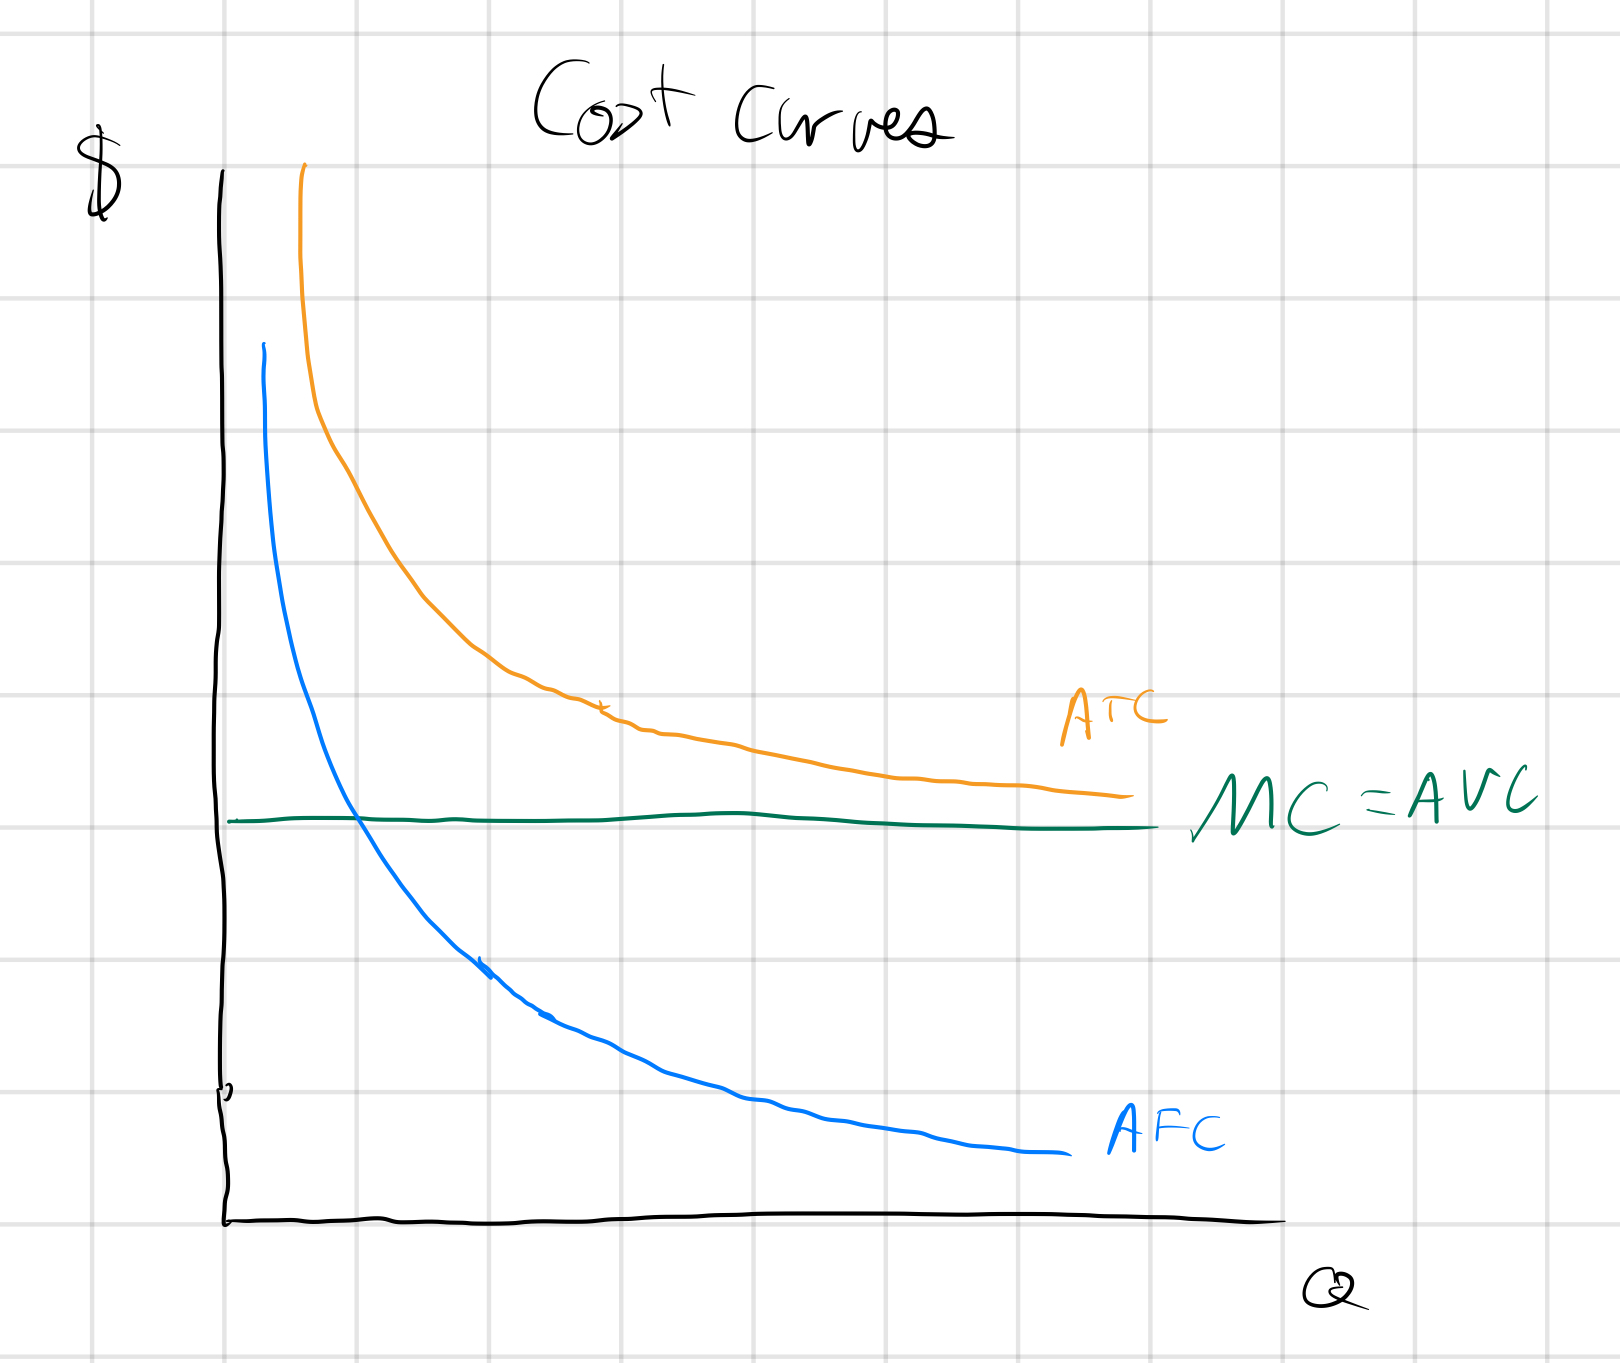
\includegraphics[width=10cm]{HW7Q2A}
\end{center}
\subsection*{Part B}
\begin{center}
	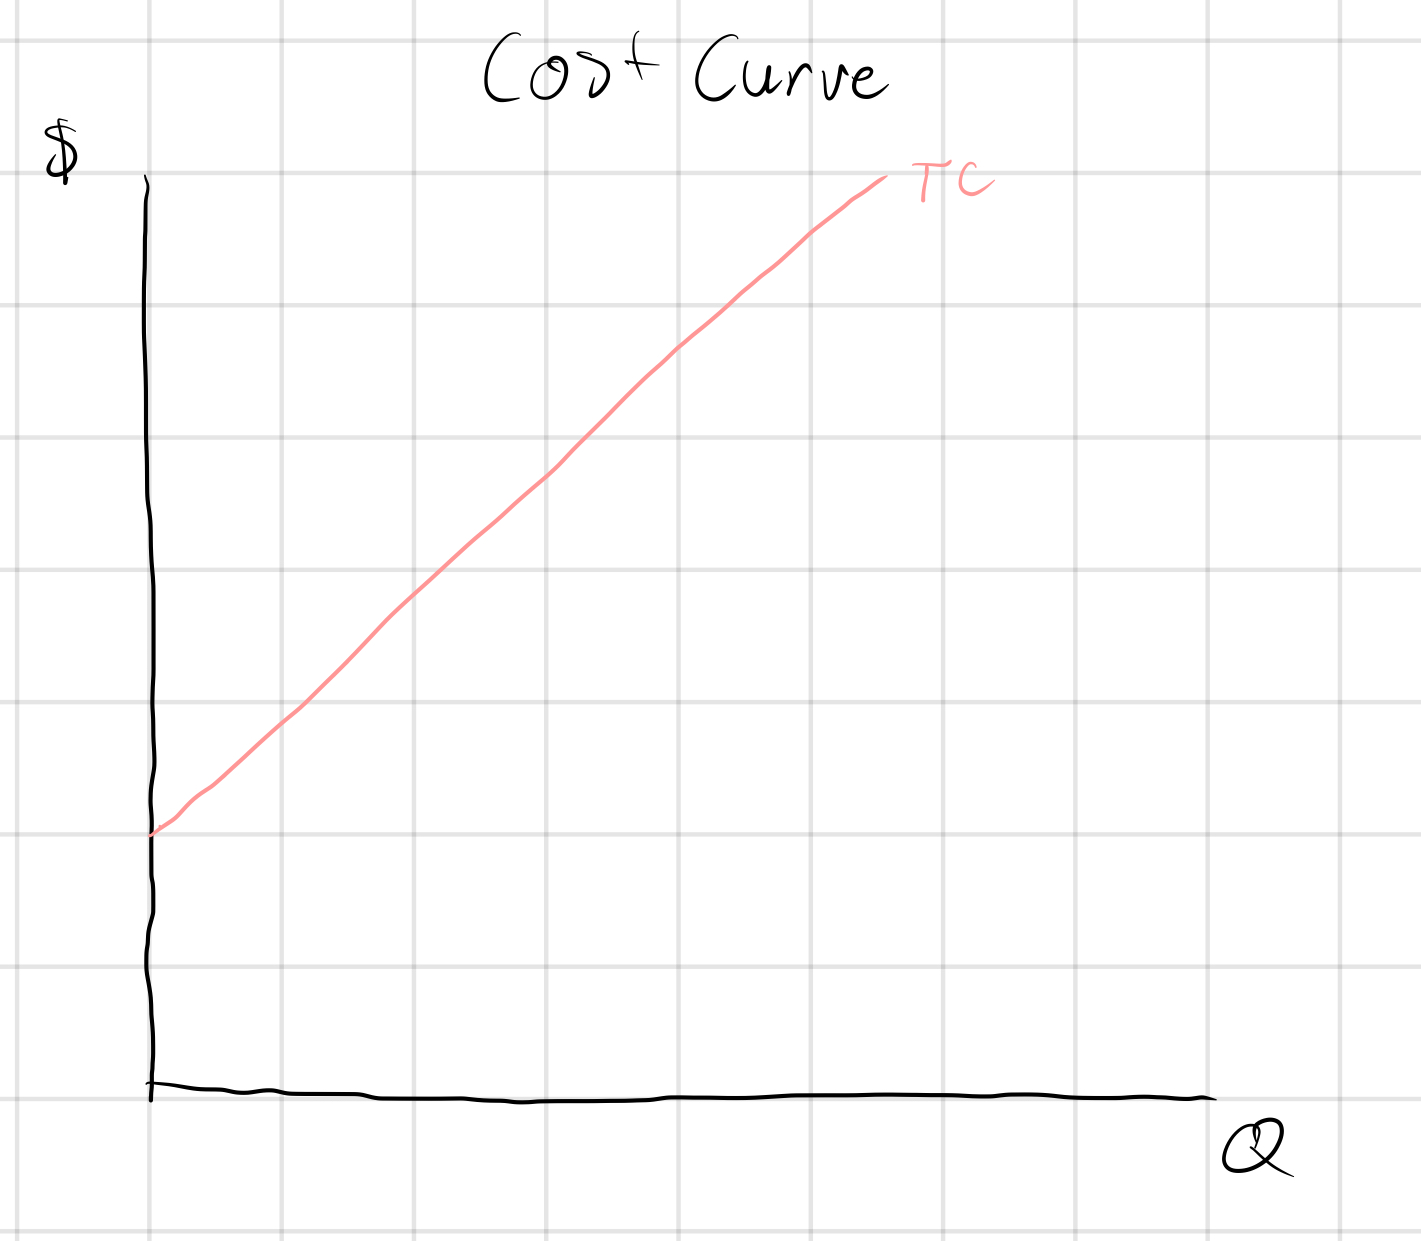
\includegraphics[width=10cm]{HW7Q2B}
\end{center}
\section{Types of Cost Curves, Mathematically}
\label{sec:Types of Cost Curves, Mathematically}
\subsection*{Part A}
\begin{align*}
	\label{eq:}
	ATC(Q) &= \frac{TC(Q)}{Q} \\
	&= \frac{288}{Q} + 3 + 2Q \\
	AVC(Q) &= \frac{VC(Q)}{Q} \\
	&= 3 + 2Q \\
	MC(Q) &= \frac{dTC}{dQ} \\
	&= 3 + 4Q
\end{align*}
\subsection*{Part B}
\begin{align*}
	\label{eq:}
	\frac{d(ATC)}{dQ} &= 0 \\
	-\frac{288}{Q^2} + 2 &= 0 \\
	Q &= 12 \\
	ATC(Q) &= MC(Q) \\
	\frac{288}{Q} + 3 + 2Q &= 3 + 4Q \\
	\frac{288}{Q} &= 2Q \\
	Q &= 12 
\end{align*}
\section{Cost Curves, Graphically}
\label{sec:Cost Curves, Graphically}
\begin{center}
	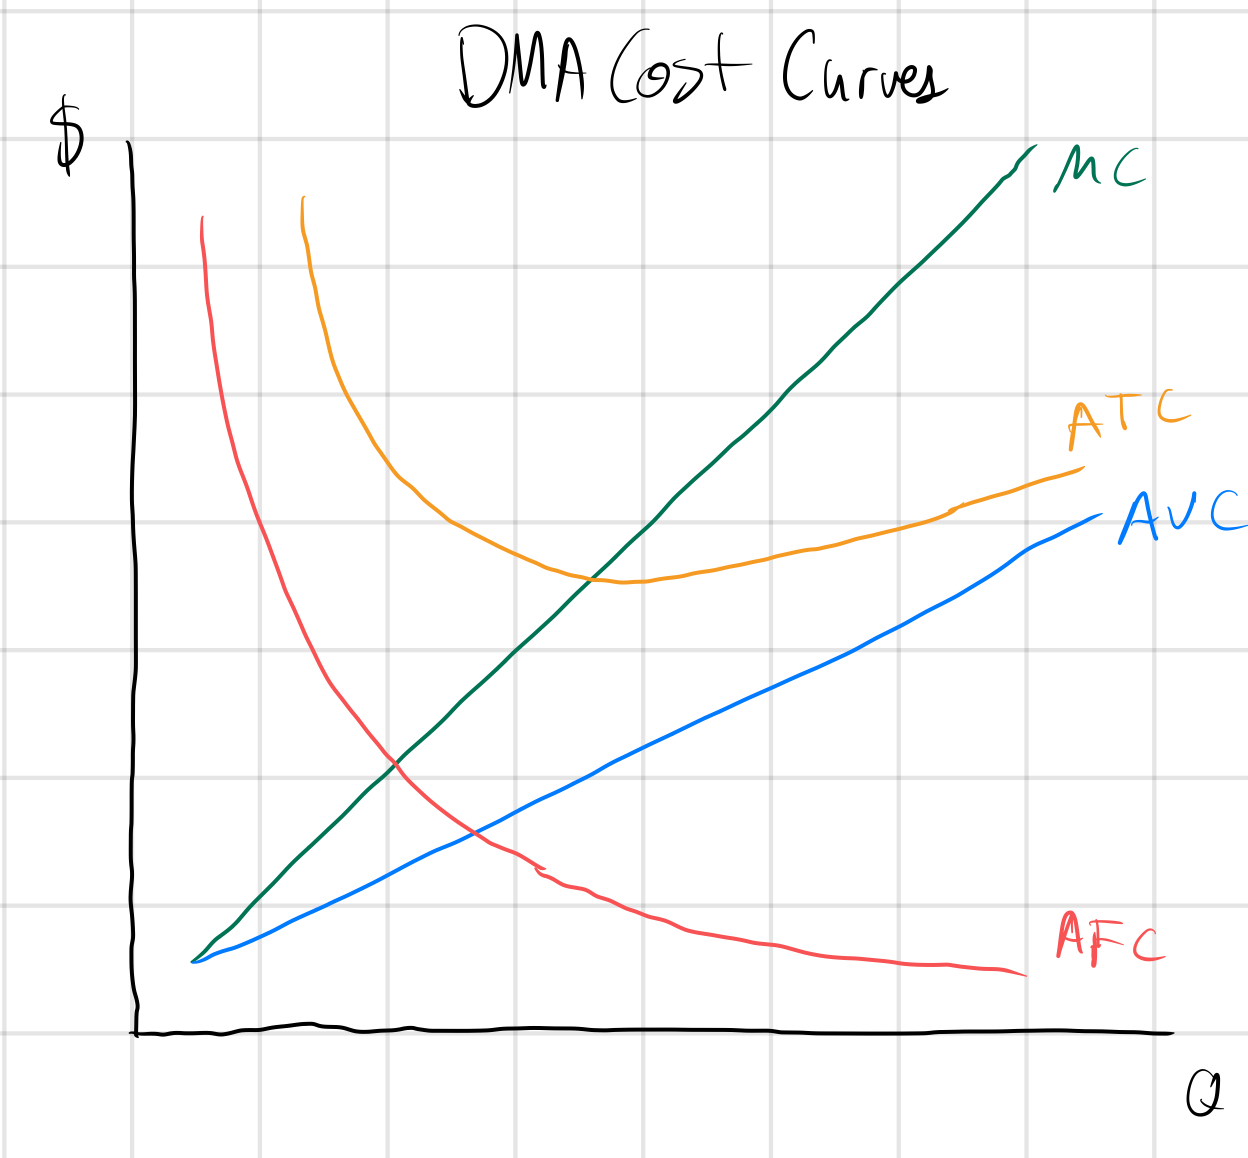
\includegraphics[width=10cm]{HW7Q4}
\end{center}
\subsection*{Part A}
\begin{center}
	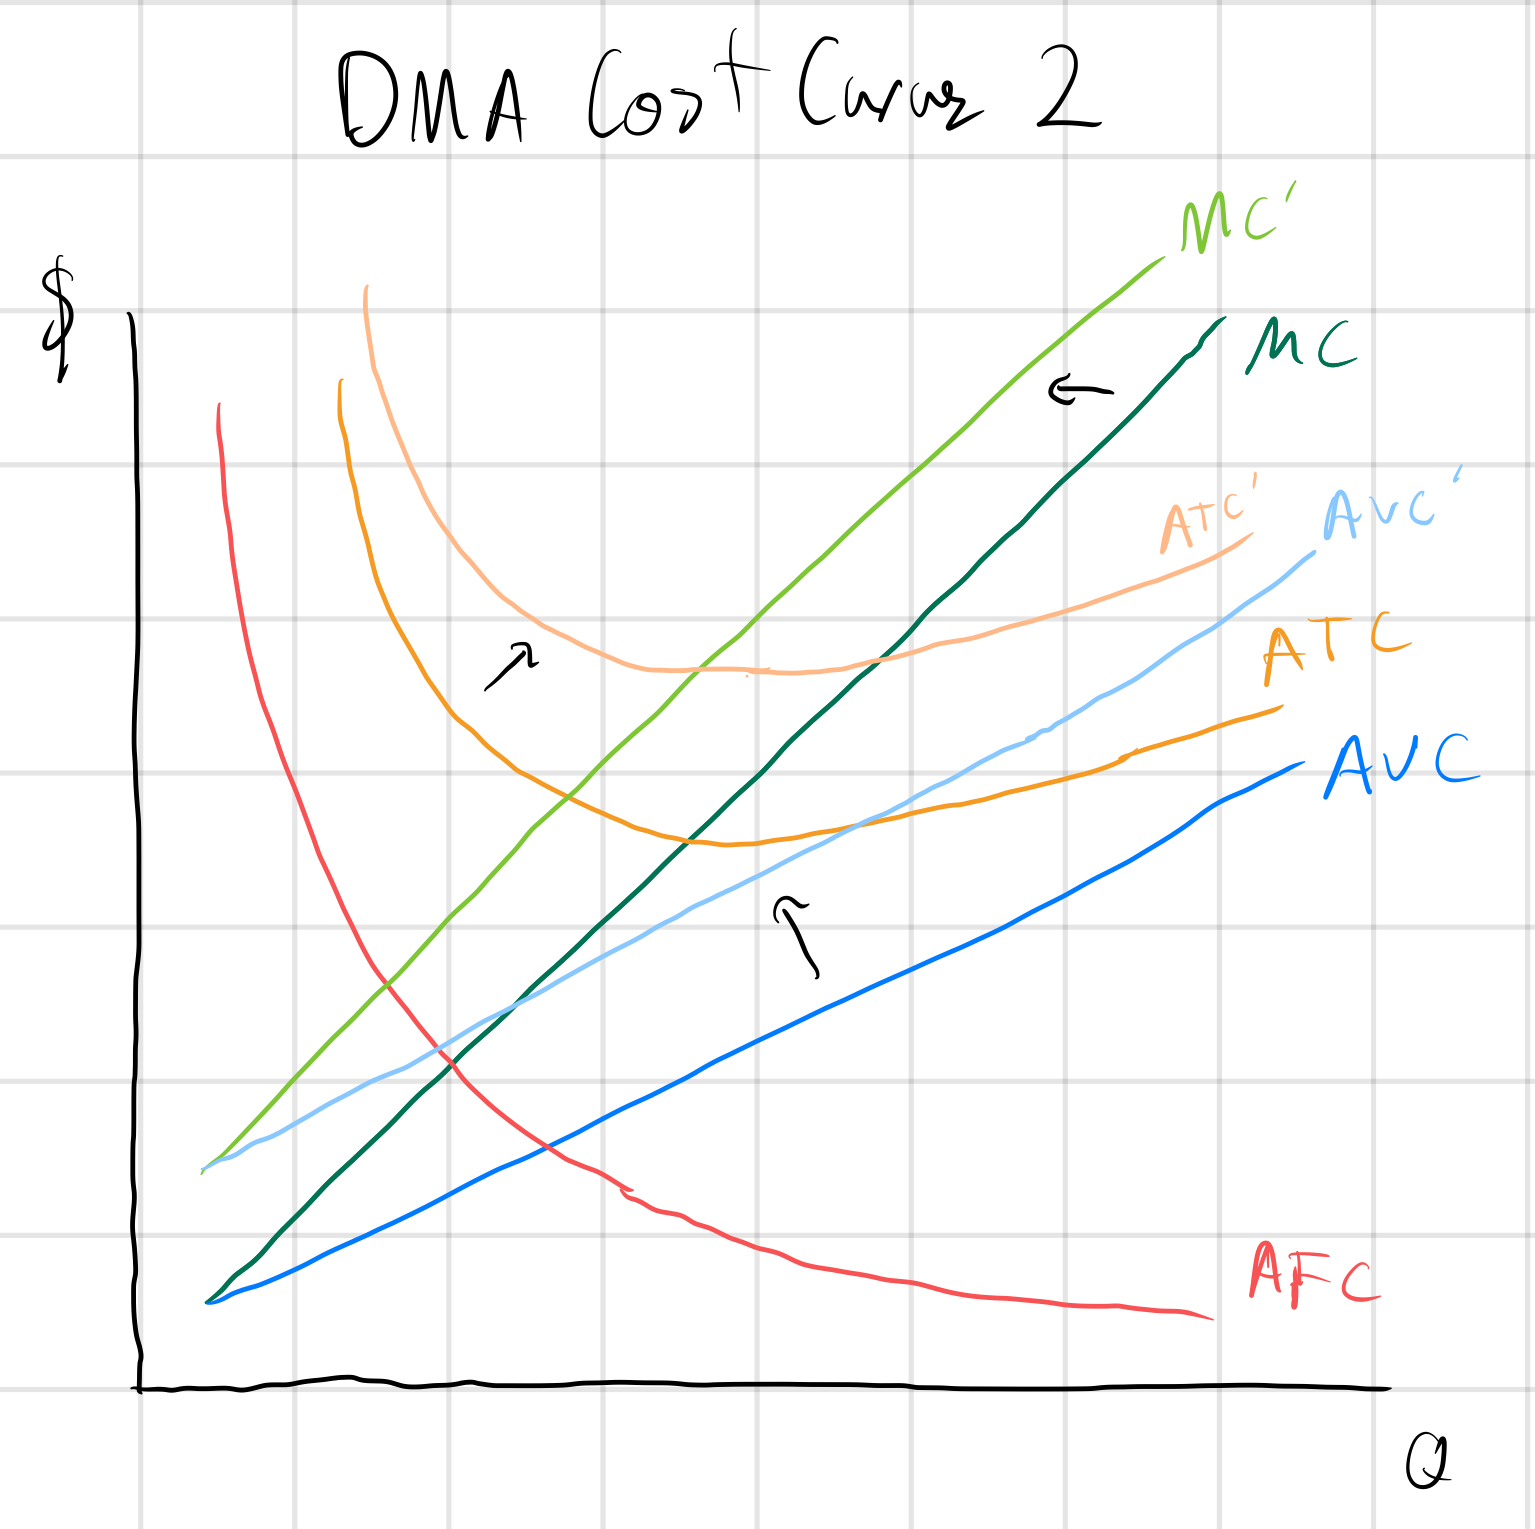
\includegraphics[width=10cm]{HW7Q4A}
\end{center}
\subsection*{Part B}
\begin{center}
	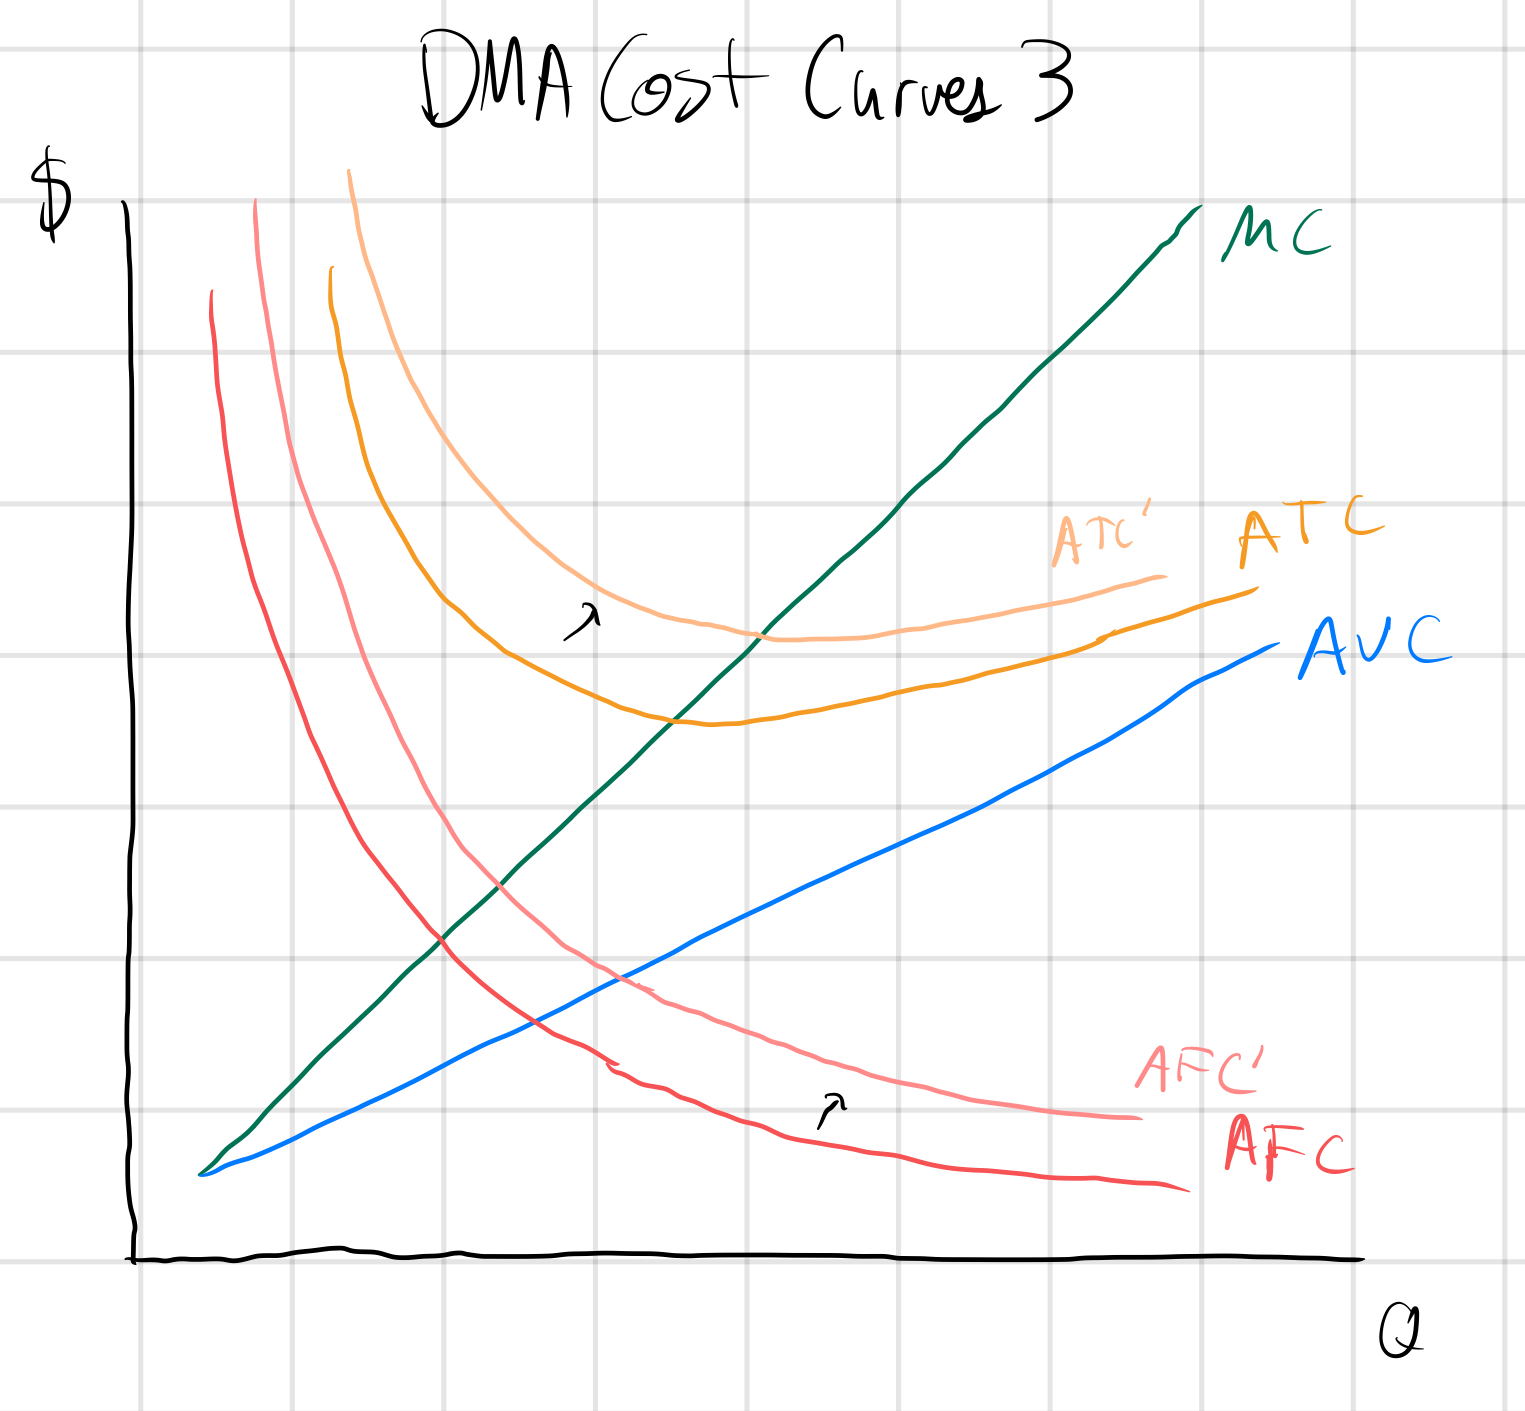
\includegraphics[width=10cm]{HW7Q4B}
\end{center}
\section{Cost Curves, Verbal Description}
\label{sec:Cost Curves, Verbal Description}
\subsection*{Part A}
\begin{align*}
	\label{eq:}
	C_{\plain{direct}} &= 200 + 30Q \\
	Q &= 5T \\
	C_{\plain{direct}} &= 200 + 150T \\
	C_{\plain{opp}} &= 50(T^2 - 3T) \\
	C_{\plain{tot}} &= C_{\plain{direct}} + C_{\plain{opp}} \\
	&= 200 + 150T + 50T^2 - 150T \\
	&= 20 + 50T^2 \\
	&= \boxed{20 + 2Q^2}
\end{align*}
\subsection*{Part B}
Marjorie's business exhibits \textbf{diseconomies of scale}, as doubling production yields greater than a doubling in costs.
\section{Conceptual Questions}
\label{sec:Conceptual Questions}
\begin{enumerate}
	\item Casey did \textbf{not} make a profit, as the opportunity cost is equal to $4\times 35 = 140$ and the direct cost was $15$, which is greater than the $150$ he received at the end of the tournament.
	\item Philo should \textbf{wait}\textemdash the \$20K spent on planting the corn is sunk costs, and the marginal revenue from harvesting the corn is only \$2 in September, while it is \$10 in May. The cost of harvesting the corn is fixed, too, so marginal revenue is higher than marginal cost in May.
\end{enumerate}
\section{Short Run Total Cost Curves}
\label{sec:Short Run Total Cost Curves}
\begin{align*}
	\label{eq:}
	Q &= \textrm{min}(0.5K,L) \\
	Q &= \textrm{min}(0.5(8),L) \\
	4 &= \textrm{min}(4,L) \\
	SRTC(Q) &= 64 + 4Q, Q\leq 4
\end{align*}
\section{Short Run Cost Functions}
\label{sec:Short Run Cost Functions}
\begin{align*}
	\label{eq:}
	Q(S,L) &= 0.1S^{\frac{1}{2}}L^{\frac{3}{4}} \\
	Q(\overline{S},L) &= 0.1(10)L^{\frac{3}{4}} \\
	&= L^{\frac{3}{4}} \\
	L &= Q^{\frac{4}{3}} \\
	L(Q) &= Q^{\frac{3}{4}} \\
	SRTC(Q) &= 
\end{align*}
\section{Short Run Total Cost Function}
\label{sec:Short Run Total Cost Function}
\subsection*{Part A}
\begin{align*}
	\label{eq:}
	Q(K,L) &= K + 2L\\
	Q(\overline{K},L) &= 20 + 2L \\
	L &= \frac{Q-20}{2} \\
	SRTC(Q) &= 800 + 10Q, Q\geq 20
\end{align*}
\subsection*{Part B}
\begin{align*}
	\label{eq:}
	STRTC(Q) &= \boxed{1000}
\end{align*}
\section{Long Run Total Costs, Standard Case}
\label{sec:Long Run Total Costs, Standard Case}
\subsection*{Part A}
\begin{align*}
	\label{eq:}
	Q &= K^{\frac{1}{2} }L^{\frac{1}{2} } \\
	MRTS_{KL} &= \frac{L}{K} \\
	\frac{L}{K} &= \frac{10}{5} \\
	L &= 2K \\
	Q &= K^{\frac{1}{2} }\left(2K^{\frac{1}{2} }\right) \\
	Q &= K\sqrt{2} \\
	K &= \frac{Q\sqrt{2}}{2} \\
	L &= Q\sqrt{2} \\
	LRTC(Q) &= 10\frac{Q\sqrt{2}}{2} + 5Q\sqrt{2} \\
	&= 10Q\sqrt{2}
\end{align*}
\subsection*{Part B}
The production function exhibits constant economies of scale as the $LRTC$ function is linear in $Q$.
\section{Deriving Total Cost Curves, Special Case}
\label{sec:Deriving Total Cost Curves, Special Case}
\begin{align*}
	\label{eq:}
	Q &= K + 10\sqrt{L} \\
	MRTS_{KL} &= \frac{1}{10\frac{1}{2\sqrt{L}}} \\
	\frac{\sqrt{L}}{5} &= 1 \\
	\sqrt{L} &= 5 \\
	L &= 25 \\
	K &= Q-50 \\
	LRTC(Q) &= \begin{cases}
		Q-50, & Q \geq 50 \\
		\left(\frac{Q}{10}\right)^2, & Q < 50
	\end{cases} 
\end{align*}
\section{Operation Decisions}
\label{sec:Operation Decisions}
\subsection*{Part A}
Since the value of $P$ is below the value of $ATC$ at 11 units, the owner will shut down in the long run.
\subsection*{Part B}
The short run loss will be equal to $(AFC)(Q^*) = (10.25-7.50)(11) = 30.25$
\subsection*{Part C}
If the price is 7, it is better for the firm to produce zero units in the short run than to produce units, as the price is below the average variable cost. If the price is 9, then it is fine for the firm to produce units in the short run as the producer surplus is positive, but in the long run the firm will shut down as 9 is still below the average total cost curve.
\section{Shutdown Decisions, Graphically}
\label{sec:Shutdown Decisions, Graphically}
\subsection*{Part A}%
\label{sub:Part A}
\begin{center}
	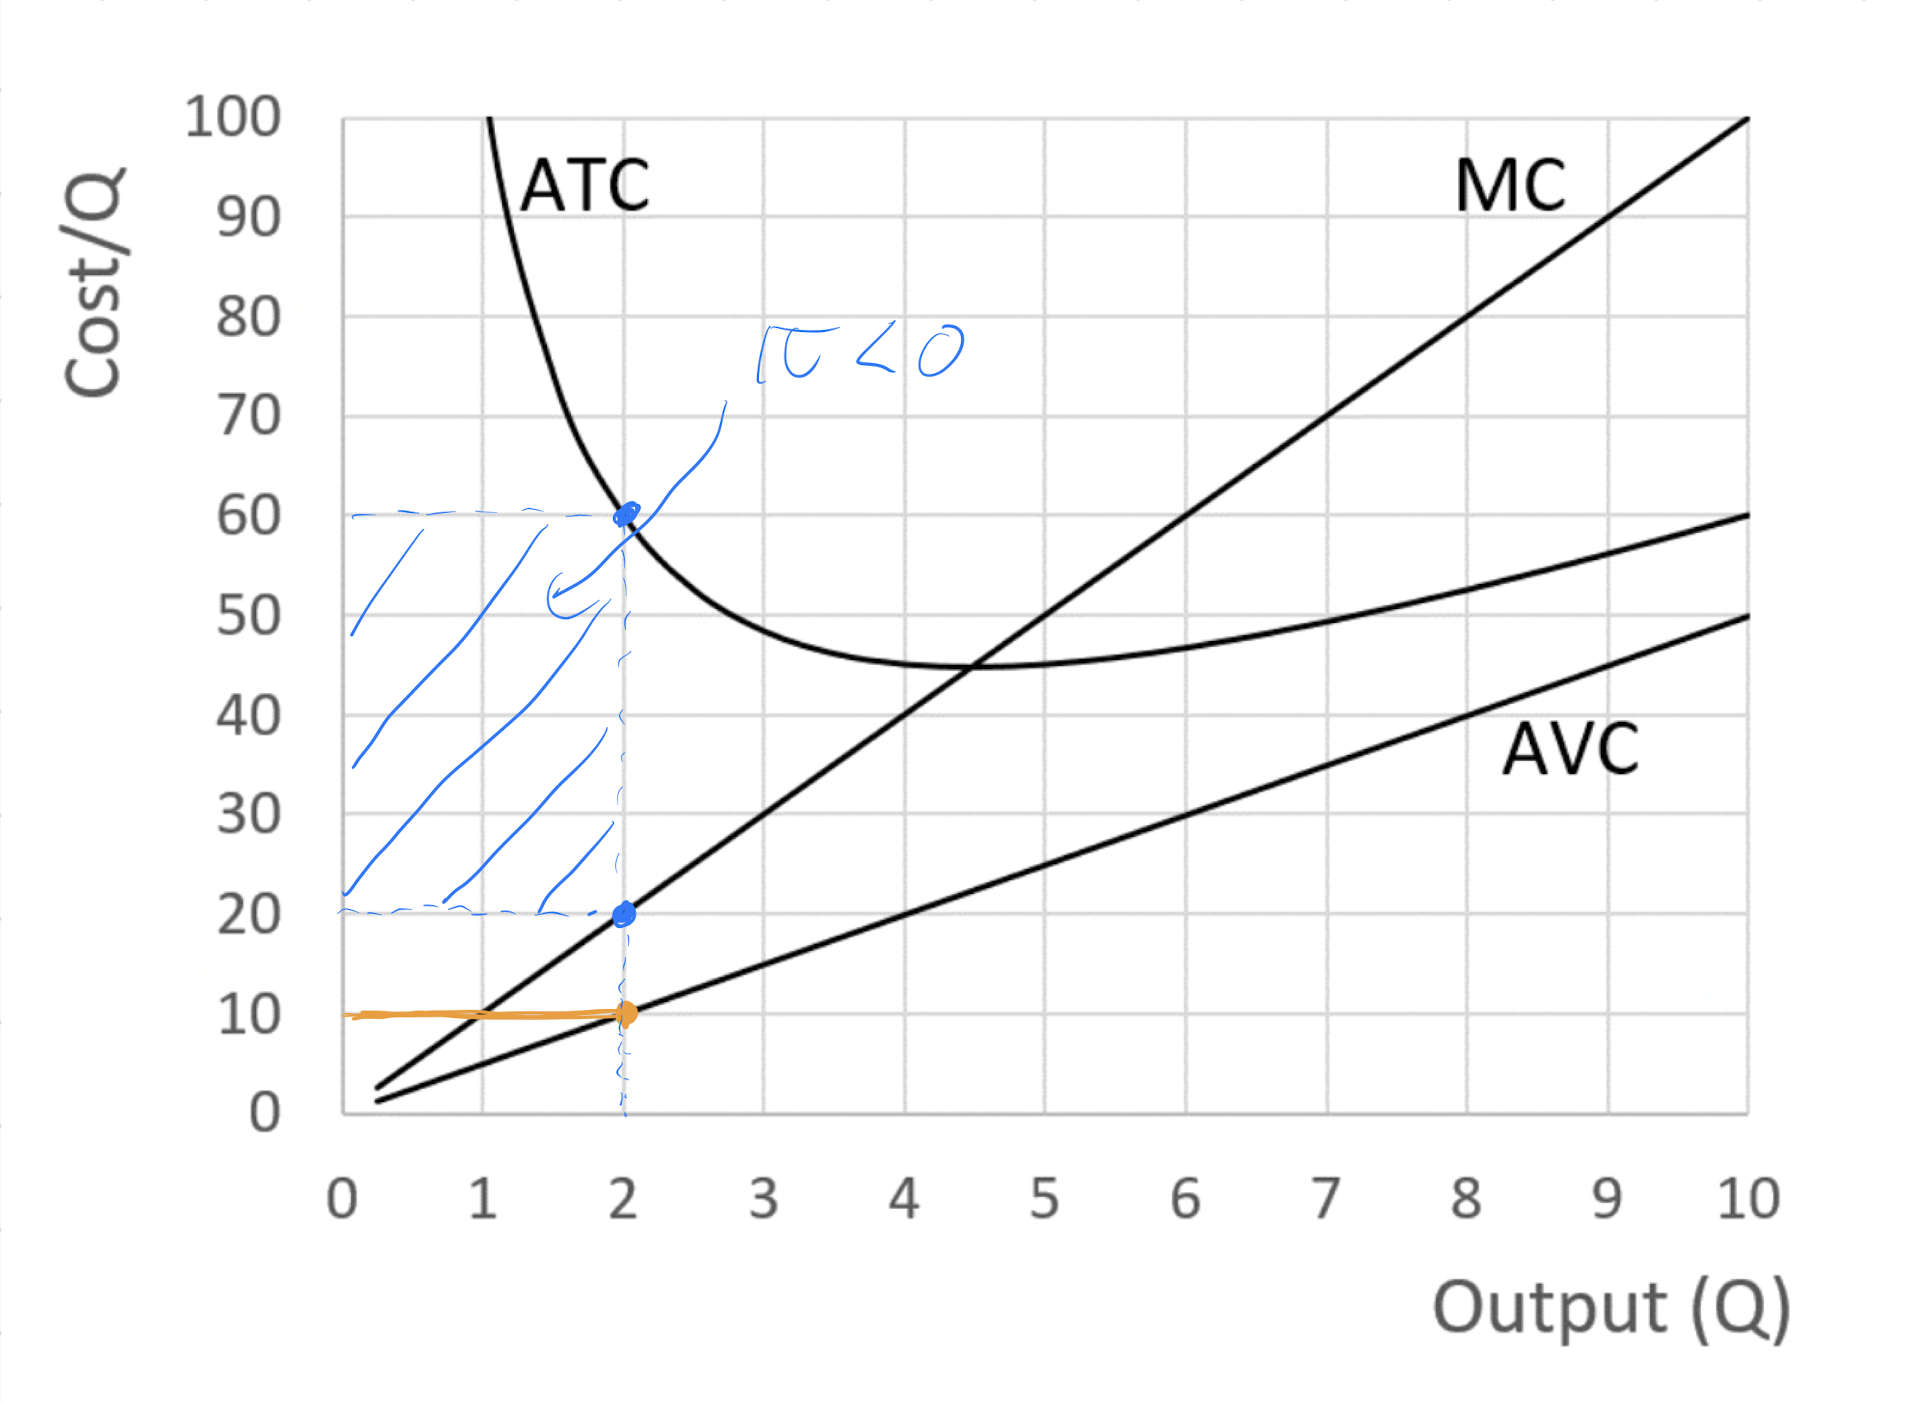
\includegraphics[width=10cm]{HW7Q13A}
\end{center}
\begin{align*}
	\label{eq:}
	\pi &= (P-ATC)(Q^*) \\
	&= (20-60)(2) \\
	&= -80
\end{align*}
\subsection*{Part B}%
\label{sub:Part B}
Lindsey \textbf{should} operate in the short run as her producer surplus ($P-AVC$) is positive.
\section{Shutdown Decisions, Math}
\label{sec:Shutdown Decisions, Math}
\begin{align*}
	\label{eq:}
	TC(Q) &= Q^3 -3Q^2 + 10Q \\
	ATC(Q) &= \frac{TC(Q)}{Q} \\
	&= Q^2 - 3Q + 10 \\
	MC(Q) &= \frac{dTC}{dQ} \\
	&= 3Q^2 - 6Q + 10 \\
	MC &= MR \\
	MR &= 10 \\
	10 &= 3Q^2 - 6Q + 10 \\
	Q(3Q-6) &= 0\\
	Q &= 2 \\
	ATC(2) &= (4)-(6) + 10 \\
	&= 8
\end{align*}
Since $MR = 10$ is greater than $ATC = 8$, The York \textbf{should} operate in the long run.
}\end{document}